%%%%%%%%%%%%%%%%%%%%%%%%%%%%%%%%%%%%%%%%%%%%%%%%%%%%%%%%
%
% Change the option between square brackets
% depending on the document you have to write:
%
% proposal    for the initial proposal
% review      for the literature review
% progress    for the progress report
% final       for the final report
% 
%%%%%%%%%%%%%%%%%%%%%%%%%%%%%%%%%%%%%%%%%%%%%%%%%%%%%%%%
\documentclass[review]{cmpreport}
\makeatletter
\input{t1pcr.fd}
\makeatother
\setlength{\footnotesep}{3ex}

% Some package I am using. You may not need them
%
\usepackage{rotating}
\usepackage{subfloat}

%\setkeys{Gin}{draft}

%%%%%%%%%%%%%%%%%%%%%%%%%%%%%%%%%%%%%%%%%%%%%%%%%%%%%%%%
%
%  Fill in the fields with:
%
%  your project title
%  your name
%  your registration number
%  your supervisor's name
%
%%%%%%%%%%%%%%%%%%%%%%%%%%%%%%%%%%%%%%%%%%%%%%%%%%%%%%%%
\title{Literature Review - Investigating The Use Of Intelligent Search In AI For Solving Problems Efficiently}

%%%%%%%%%%%%%%%%%%%%%%%%%%%%%%%%%%%%%%%%%%%%%%%%%%%%%%%%
%
% The author's name is ignored if the following command 
% is not present in the document
%
% Before submitting a PDF of your final report to the 
% project database you may comment out the command
% if you are worried about lack of anonimity.
%
%%%%%%%%%%%%%%%%%%%%%%%%%%%%%%%%%%%%%%%%%%%%%%%%%%%%%%%%
\author{Luke Garrigan}


\registration{100086495}
\supervisor{Dr Pierre Chardaire}
%%%%%%%%%%%%%%%%%%%%%%%%%%%%%%%%%%%%%%%%%%%%%%%%%%%%%%%%
%
% Fill in the field with your module code.
% this should be:
%
% for BIS            -> CMP-6012Y
% for BUSINESS STATS -> CMP-6028Y
% for other students -> CMP-6013Y
%
%%%%%%%%%%%%%%%%%%%%%%%%%%%%%%%%%%%%%%%%%%%%%%%%%%%%%%%%
\ccode{CMP-6012Y}


\summary{
This document explains how to use the class file \texttt{cmpreport.cls} to write your reports.
The class file has been designed to simplify your life; many things are done for you. As a consequence
some commands presented here are specific to the class file whether they are new commands or customized versions
of commonly known \LaTeX\ commands.
}

\acknowledgements{
This section is used to acknowledge whoever's support and contribution.
The command that introduces it is ignored in the project proposal, literature review and progress report. It is used in the
final report,  but  is not compulsory. If you do not
have an acknowledgements command in your preamble then there
won't be any acknowledgement section in the document produced. \emph{Abstract} and \emph{Acknowledgements} sections should fit on the same page. 
}

%%%%%%%%%%%%%%%%%%%%%%%%%%%%%%%%%%%%%%%%%%%%%%%%%%%%%%%%%%%%%%%%%%
%
% If you do not want a list of figures and a list of tables
% to appear after the table of content then uncomment this line 
%
% Note that the class file contains code to avoid
% producing an empty list section (e.g list of figures) if the 
% list is empty (i.e. no figure in document).
%
% The command also prevents inserting a list of figures or tables 
% anywhere else in the document
%
% Some supervisors think that a report should not contain these
% lists. Please ask your supervisor's opinion.
%
%%%%%%%%%%%%%%%%%%%%%%%%%%%%%%%%%%%%%%%%%%%%%%%%%%%%%%%%%%%%%%%%%%
%\nolist,

%%%%%%%%%%%%%%%%%%%%%%%%%%%%%%%%%%%%%%%%%%%%%%%%%%%%%%%%%%%%%%%%%%
%
% Comment out if you want your list of figures and list of
% tables on two or more pages, in particular if the lists do not fit 
% on a single page.
%
%%%%%%%%%%%%%%%%%%%%%%%%%%%%%%%%%%%%%%%%%%%%%%%%%%%%%%%%%%%%%%%%%%
\onePageLists

\begin{document}


\section{Introduction}




A classic example in the AI literature of pathfinding problems are the sliding-tiles puzzles such as the $3\times3$ Eight Puzzle, the $4\times4$ 15 puzzle and the $5\times5$ twenty-four puzzle. The Eight Puzzle consists of a $3\times3$ grid with 8 numbered square tiles and 1 blank. The blank is used to slide other tiles in which are horizontally or vertically adjacent into that position in an attempt to reach the goal state. The objective of the puzzle is to move the tiles from a set composition to a goal configuration, which is with the numbers in ascending order from 1 to 8. In terms of AI search algorithms the goal would be to complete the puzzle in the minimum number of moves.  

\begin{figure}[ht]
	\centering
	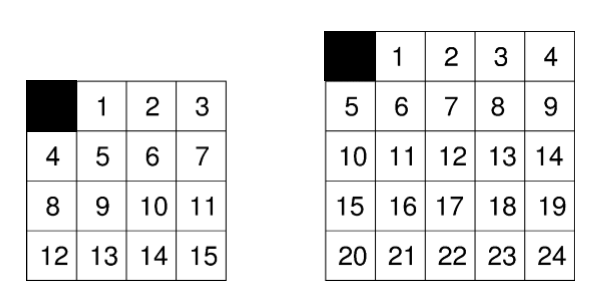
\includegraphics[width=0.5\textwidth]{sliding_tile}
	\captionsetup{justification=centering}
	\caption{The goal states of the Fifteen and Twenty-Four Puzzles}
\end{figure}
The Rubik's Cube is also another classic example in AI literature of pathfinding problems. combinatorial puzzle. Each $3\times3$ plane can be rotated 90 or 180 degrees, clockwise or anticlockwise. The goal of the game is to have all 6 sides showing only one colour. The $3\time3\time3$ Rubik's Cube contains about $4.3252\times10^{19}$ different reachable states. There are 20 movable sub cubes, or cubies, which can be divided into eight corner cubies, with three faces each, and twelve edge cubies, with two faces each. There are $88,179,840$ different positions and orientations of the corner cubies, and the number of moves needed to solve just the corner cubies ranges from zero to eleven. \citep{DBLP:journals/corr/abs-1107-0050}.

\begin{figure}[ht]
	\centering
	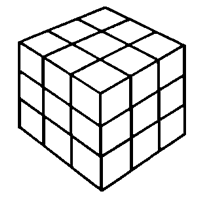
\includegraphics[width=0.3\textwidth]{rubiks}
	\captionsetup{justification=centering}
	\caption{The Rubik's Cube}
\end{figure}

I will begin by describing the problem-space model on which search algorithms are based. Brute-force searches are then considered including breadth-first, depth-first and depth-first iterative-deepening. I also cover heuristic searches such as the A* algorithm and iterative-deepening A*.


\section{Problem Space Model} \label{sec1}

The problem space is the entire range of components that exist in the process of finding a problem's solution. So in terms of AI a problem space is the environment in which a search takes place.  \citep{Newell:1972:HPS:1095704}. A problem space consists of a set of states of a problem and a  set of operators in which change the state. In the tile problem the operators move a tile into the blank position which in turn alters the state. States are the different possible permutations of the tiles in the grid. A problem instance is a problem space together with an initial state and a goal state, in the sliding-tile puzzle the initial state would be the original randomised configuration of the tiles, and the goal state would be the tiles in an ascending order with the blank tile at the top left. \citep{DBLP:journals/mima/Korf95}.
\section{Search} \label{sec1}
A search algorithm is a series of steps that can be used to find the location or the path of a desired state. In most scenarios there will be additional constraints that will need to be fulfilled such as the amount of time taken to reach the desired state, amount of memory available, maximum number of moves. An example would be for finding a route between two cities, it is likely that for this scenario, distance and time will need to be considered in order to find the most efficient route. Because of the vast number of applications that are in need of search algorithms and the considerations discussed, explains the reasoning for the extensive number of alternative searches. Each algorithm comes with their own advantages and disadvantages, which is why it is essential to consider which algorithm is the most suited for the given task.

\subsubsection{Brute-Force Search} \label{sec1}
Brute-force search is a general problem-solving technique that consists of systematically enumerating all the possible options for a given solution and checking to see whether that given option satisfies the problem's statement. All that is required to execute a brute-force is some legal operators, an initial state and an acknowledged goal state. Examples of brute-force search that I have covered below are breadth-first search, depth-first search and depth-first iterative-deepening.
\subsubsection{Breadth-First Search}
Breadth-first search expands the nodes in a tree in the order of their given distance from the root, so it expands all the neighbouring nodes before going to the next level of the tree. Because the algorithm doesn't trawl to the deeper levels of the tree without first expanding the lower levels, it ensures the finding of the shortest path. The amount of time used by breadth-first search is linear to the number of nodes expanded, since each node can be generated in constant time, and is a function of the branching factor $b$ and the solution depth $d$. Since the number of nodes at level $d$ is $b^d$, the total number of nodes generated in the worst case is $O(b^d)$. \citep{DBLP:journals/mima/Korf95}.

\begin{figure}[ht]
	\centering
	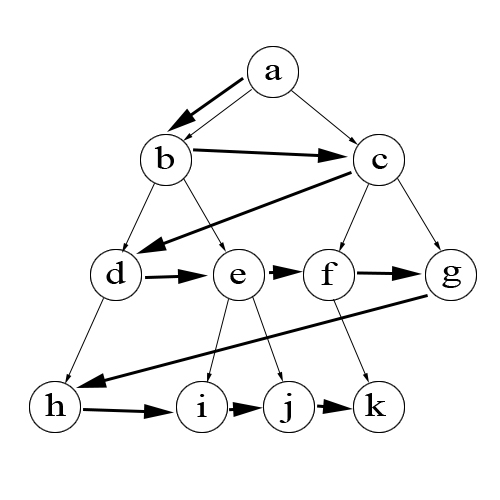
\includegraphics[width=0.5\textwidth]{breadth_first}
	\captionsetup{justification=centering}
	\caption{Breadth-first Search}
\end{figure}
Breadth-first search will likely exhaust the memory available on most machines in a matter of minutes as the memory is proportional to the number of nodes stored and each level of the tree must be saved in order to generate the next level giving it its complexity of $O(b^d)$.
\subsubsection{Depth-First Search}
Depth-first search (DFS) addresses the limitations of breadth-first by always generating next a child of the deepest unexpanded node. Breadth-first search manages the list as a first-in first-out queue, whereas depth-first search treats the list as a last-in first-out stack. Depth-first search is implemented recursively, with the recursion stack taking the place of an explicit node stack. Given a starting state, depth-first search stores all the unvisited children of that state in a stack. It then removes the top state from the stack and adds all of the removed states children to the stack. Depth first search generates a long sequence of moves, only ever reconsidering a move when it reaches the end of a stack, this can become a serious problem given a graph of significant size and there's only one solution, as it may end up exploring the entire graph on a single DFS path only to find the solution after looking at each node. Worse, if the graph is infinite the search might not terminate. Unlike breadth-first search if there a multiple ways to reach a goal state Depth-first search will not necessarily find the shortest path. Finding the shortest path however is all dependent on the application, If for example you wanted to find the solution to the sliding tile puzzle in the minimum number of moves, depth-first search wouldn't be the first choice. \citep{DBLP:journals/mima/Korf95}.
\begin{figure}[ht]
	\centering
	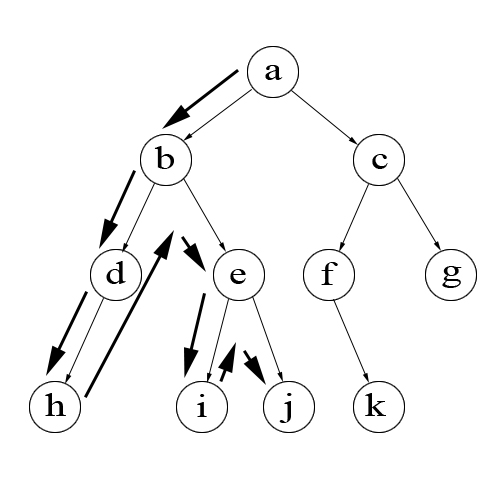
\includegraphics[width=0.5\textwidth]{depth_first}
	\captionsetup{justification=centering}
	\caption{Depth-first Search}
\end{figure}

\subsubsection{Depth-First Iterative-Deepening}
Depth-First Iterative-Deepening (DFID) is an extension of depth-first search, it combines the best features of breadth-first search and depth-first search. DFID has a maximum depth, so it searches all possibilities up to a certain depth and if it doesn't find the goal state it increases the search depth. DFID performs depth-first search to depth one, then starts over and executes a depth-first search to depth two and continues deeper and deeper until a solution is found. The complexity of DFID is only O(d) where d is the depth, this is because at a given point it is executing only a depth-first search and saving only a stack of nodes. DFID ensures that the shortest path to the goal state will be found as does breadth-first search. \citep{DBLP:conf/otm/MeissnerB11}.

\subsubsection{Combinatorial Explosion}
The prime complication with brute-force search algorithms is that their time complexities grow exponentially along with the problem size. This is what is known as a combinatorial explosion and is the fundamental reason for the limited use of the brute-force search on sizable problems. This is why the sliding-tile puzzle is so interesting, the $3\times3$ Eight Puzzle has $10^5$ states and can be solved easily with brute-force search, The Fifteen Puzzle has $10^{13}$ states and cannot be solved on most machines today in a brute-force fashion. The Twenty-Four Puzzle contains $10^{25}$ states in relation. 

This is not to say that these puzzles cannot be solved optimally. For the sliding-tile puzzles, currently the largest size problem for which random instances can be solved optimally is the $5\times 5$ Twenty-Four Puzzle. For Rubik's Cube, the classic $3 \times 3 \times 3$ is the state of the art. The next research challenge is to optimally solve random instances of the $6 \times 6$ Thirty-Five Puzzle, or the $4 \times 4 \times 4$ Rubik's Cube. Since these represent enormous increases in the sizes of the corresponding search spaces, for the sliding-tile puzzles at least one can consider intermediate problems such as the $5 \times 6$ Twenty-Nine Puzzle. \citep{DBLP:journals/aicom/BorrajoFKLLRS14}. 

\subsection{Heuristic Search} \label{sec1}
Heuristics are generally used in order to improve search efficiency. A heuristic is a method that might not always find the best solution but it will guarantee to find a good solution in a reasonable time. The idea behind a heuristic function is that it sacrifices the completeness in order to increase efficiency. They are usually utilised in solutions in which may take infinite time or a very long time to compute. \citep{DBLP:conf/ai/2014}.

\subsubsection{Heuristic Evaluation Functions}
A common heuristic function for the sliding-tile puzzle is called Manhattan distance. The Manhattan distance is the distance between two points in a grid, based on a strictly horizontal and/or vertical path and summing these values over all tiles. For a fixed goal state, a heuristic evaluation is a function of a node, $h(n)$ in which estimates the distance from the node to said goal state.


Heuristic evaluation functions estimate the actual cost with very little computational power, thus very compelling. The complexity of the Manhattan Distance is proportional to the number of tiles between the initial state and the goal state. Most heuristic functions are lower bounds on the actual cost deeming them admissible. A heuristic function is said to be admissible if it never overestimates the cost of reaching the goal, i.e the cost it estimates to reach the goal from the initial state is not higher than the lowest possible cost from said point. The Manhattan distance is a lower bound for the number of moves required to solve an occurrence of the sliding-tile puzzle, since every tile must move at least as many times as its distance to its goal position. \citep{DBLP:conf/ccgrid/LinnertSB14}.
\subsubsection{A* Algorithm}
A* search is a combination of lowest-cost-first and best-first searches that considers both path cost and heuristic information in its selection of which path to expand. For each path on the frontier, A* uses an heuristic of the path cost from a start node to a goal node constrained to start along that path. This allows A* search to ensure the prioritisation of states in which are more likely to result in a low-cost goal state. The calculation of the heuristic value is dependent on the problem that is being solved. For example, for problems which aim to reach a location the Euclidean distance between the state and the goal is often used as the heuristic. 
The A* algorithm uses $cost(p)$, the cost of the path found, as well as the heuristic function $h(p)$, the estimated path cost from the end of $p$ to the goal. As A* uses admissible heuristic it will always find solutions in the order of their cost. \citep{DBLP:journals/ker/Brewka96}.  A* uses breadth-first traversal thus uses a large chunks of memory in comparison to applications that use depth-first traversal. The performance of A* is also heavily reliant on the accuracy of the heuristic.

\subsubsection{Iterative-Deepening-A*}
Iterative-deepening-A* (IDA*) eradicates the memory complication of A* by using depth-first traversal, without sacrificing solution optimality at the cost of increasing the time taken. Each iteration of A* is a complete depth-first search that keeps track of the cost, $f(n) = g(n) = h(n)$, of each node generated. If an expanded node's cost generated exceeds a threshold for that iteration, its path is cut off and the search backtracks before continuing. IDA* ranks states the same way as A*: The expected cost of a state is the cost of reaching said state and the heuristic's estimate of the cost of reaching the nearest goal state. The maximum expected cost is assigned to the heuristic cost of the starting state, states in which have a lowest cost than the starting state are traversed and states with a higher expected cost are discarded. 


If IDA* has searched all states lower than the current maximum without finding the goal state then it increases the maximum to the lowest value of the discarded states and begins the search again. The goal state is admissible, the current maximum cost will never be higher than the lowest cost solution, thus IDA* with an admissible heuristic will always find the lowest cost solution.  IDA* searches many nodes multiple times thus is slower than A*. Hence, A* should be used on smaller applications that aren't going to have memory issues.

\subsubsection{Recursive Best-First Search}
Recursive best-first search (RBFS) is a best-first search that runs in space that is linear in the maximum search depth, regardless of the cost function used. Even with an admissible cost function, RBFS generates fewer nodes than IDA*, and is generally superior to IDA*, except for a small increase in the cost per node generation overhead. \citep{DBLP:journals/mima/Korf95}. The overhead of RBFS depends on how widely the promising nodes are separated in the search tree. \citep{Hatem:2015:RBS:2887007.2887167}.
The main advantage of RBFS over IDA* is that in RBFS new nodes are expanded in a best-first order even if the f-function is not monotonically increasing. By contrast IDA* expands new nodes in a best-first only for monotonically increasing f-functions. Due to their linear-space complexity both algorithms suffer from the same problem of not being able to detect duplicates. \citep{DBLP:conf/socs/Felner15}. 


RBFS stores the complete path to the current node as well as all the immediate siblings, along with the cost of the best node in the subtree explored below each sibling. If the cost of the expanded node exceeds that of a previous node in a different part of the tree, the algorithm backs up to their deepest common ancestor and continues to search in a new direction. 

\section{Project Plan}
I will be focusing on the $4\times4$ and $5\times5$ sliding puzzles because they require a heuristic search algorithm such as A*, whereas a $3\times3$ sliding puzzle could be solved with brute force, as it only has a total of 181,440 states and can be solved optimally with a breadth-first search. I will be testing and evaluating different types of heuristics for this given problem starting off with the Manhattan distance. 

I will also be testing the linear-conflict heuristic which has a significant improvement over the Manhattan distance, as it considers the goal row or column, but reversed relative to each other. What this means is that two tiles $X$ and $Y$ are in linear conflict if $X$ and $Y$ are in the same line as well as the goal positions, $Y$ is to the left of $X$ and goal position of $Y$ is to the right of goal position $X$.

The main risks which I face in tackling this project are based primarily around the time allocated. I have many algorithms which I want to design, implement and experiment for both the sliding tile puzzle and the Rubik's Cube, that I may run into trouble with time and struggle to finish certain algorithms. I have prepared for this and set out a priority ordered list for the algorithms which I will develop based upon. 

As shown in Table 1 the lower the number the higher the priority, so the algorithms with higher priority will be developed and tested first. In developing this prioritisation system I should be able to get the core components necessary for analysis and testing. I am focusing primarily on the algorithms which have been proved to have the best outcome in terms of completing the puzzles in the minimum number of moves and computing cost. With the guidelines set in terms of prioritisation I still may run into difficulties completing the algorithms but this will at least allow me to get the most important ones done first.




\begin{table}[ht]
	\caption{Algorithm Priority Table}
	\begin{center}
		\begin{tabular}{clr} \hline
			Algorithm & Sliding Tile & Rubiks Cube \\ \hline
			Iterative deepening A*  & 1 & 1 \\
			Single-source shortest-path & 3 & 3 \\ 
			A* with Recursive Best First Search & 2 & 2 \\ 
			Memory Bounded A* & 3 & 3 \\ \hline
		\end{tabular}
	\end{center}
\end{table}

With the structure in place it could also allow time for the development of my own algorithms for completing the puzzles. This isn't something I am going to allocate a specific time to do as the possibilities are quite extensive. It is a component of the project in which I will consider throughout design and development as I build up the knowledge of the benefits and flaws of certain algorithms.

In the development of this project I may gain an alternative perception of prioritisation for the list of algorithms, in which will result in an adjustment of the project plan and Gantt chart. However as of now in terms of the papers that I've read I have chosen to prioritise the most efficient algorithms.   

I will be implementing the algorithms in Prolog which is a general-purpose logic programming language associated with artificial intelligence.

\section{Defining Terms}


\begin{itemize}
	\item \textbf{Admissible}: A heuristic is admissible if it never overestimates the distance from a given state to the goal. It is admissible if it always find an optimal solution to a problem if one exists.
	\item \textbf{State}: A configuration of a given problem such as the positioning of the tiles in the sliding tile puzzle.
	\item \textbf{Search Tree}: A problem-space graph which doesn't contain cycles.
	\item \textbf{Node expansion}: Generation of all children of a given state.
    \item \textbf{Monotonically}: a monotonic function (or monotone function) is a function between ordered sets that preserves or reverses the given order.
    \item \textbf{Depth}: The length of a shortest path from the initial state to a goal state
\end{itemize}
\clearpage
\bibliography{bibfile}


\appendix
\clearpage






\end{document}

